\adparagraph{nDCG}
Figure \ref{fig:ndcg} shows the nDCG score for BC, \MC, SF, and Avg. For nDCG a higher score is better.
All methods see a sharp drop off in the quality of their recommendations as the group sizes increase.
As shown in Table \ref{tbl:ndcg}, BC drops the most in the jump from 4 to 8 group members, however it also have the best results, and outperforms all other methods across all group sizes.
\MC is the second best by only a few percentage points and follows the same trend and quickly plateaus in score.
One outlying case SF starts out close to Avg for a group size of four, but retains a higher score and is closer to BC and \MC as the size increases.
Avg is the worst performing overall.

\begin{figure}[H]
	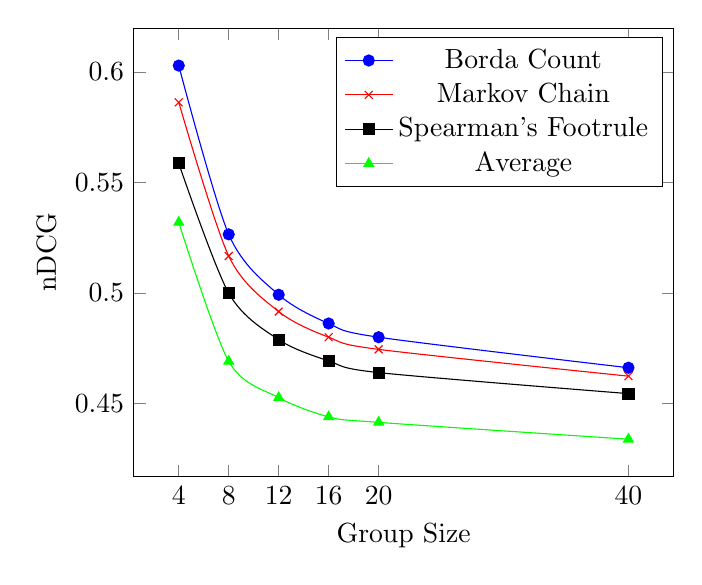
\begin{tikzpicture}
	\begin{axis}[
	xlabel=Group Size,
	ylabel=nDCG,
	xtick = {4,8,12,16,20,40}]
	\addplot[smooth,mark=*,blue] plot coordinates {
		(4,0.6028)
		(8,0.5265)
		(12,0.4992)
		(16,0.4862)
		(20,0.48)
		(40,0.4662)
	};
	\addlegendentry{Borda Count}

	\addplot[smooth,color=red,mark=x] plot coordinates {
		(4,0.5862)
		(8,0.5167)
		(12,0.4916)
		(16,0.48)
		(20,0.4745)
		(40,0.4624)
	};
	\addlegendentry{Markov Chain}
	
	\addplot[smooth,color=black,mark=square*] plot coordinates {
		(4,0.5586)
		(8,0.4999)
		(12,0.4789)
		(16,0.4693)
		(20,0.464)
		(40,0.4545)
	};
	\addlegendentry{Spearman's Footrule}
	
	\addplot[smooth,color=green,mark=triangle*] plot coordinates {
		(4,0.5319)
		(8,0.4691)
		(12,0.4527)
		(16,0.444)
		(20,0.4415)
		(40,0.4339)
	};
	\addlegendentry{Average}
	
	\end{axis}
	\end{tikzpicture}
	\caption{Results for nDCG test}\label{fig:ndcg}
\end{figure}

Another trend is observable in Table \ref{tbl:ndcg}. The highest scoring method is also dropping the most in score, aside from Avg from group size 4 to 8. This effect is visible on all group sizes for all methods.

\begin{table}[H]
	\centering
	\begin{tabular}{|l|lllll|}\hline
		& 4 to 8 & 8 to 12 & 12 to 16 & 16 to 20 & 20 to 40 \\\hline
		BC 	& 12.66	& 5.19	& 2.6	& 1.28	& 2.88 \\
		MC  & 11.86	& 4.86	& 2.36	& 1.15	& 2.55 \\
		SF  & 10.51	& 4.20	& 2.00	& 1.13	& 2.05 \\
		Avg	& 11.81	& 3.50 	& 1.92	& 0.56	& 1.72 \\ \hline
	\end{tabular}
	\caption{Percentage decrease between the groups for nDCG}
	\label{tbl:ndcg}
\end{table}

The p-values for the t-test for nDCG is shown in Table \ref{tbl:ndcg_ttest}. Our paired t-tests show that all results for the nDCG measure are statistically different from each other.

Any zeros in the table are considered to be so small that it was rounded down and is of some small non-zero value.

\begin{table}[H]
	\centering
	\begin{tabular}{|l|llllll|}\hline
		& 4 & 8 & 12 & 16 & 20 & 40 \\\hline
		BC/MC	& $3e^{-270}$	& $3e^{-234}$	& $2e^{-220}$	& $4e^{-218}$	& $1e^{-213}$ & $3e^{-205}$ \\
		BC/SF	& $0$	& $2e^{-296}$	& $7e^{-272}$	& $4e^{-249}$	& $1e^{-237}$ & $1e^{-227}$ \\
		BC/Avg	& $2e^{-310}$	& 0 & 0	& 0	& 0 & 0 \\
		MC/SF	& $2e^{-203}$	& $2e^{-166}$ 	& $3e^{-142}$	& $2e^{-129}$	& $1e^{-130}$ & $2e^{-133}$ \\
		MC/Avg	& $5e^{-228}$	& $5e^{-273}$ 	& $3e^{-278}$	& $5e^{-289}$	& $1e^{-309}$ & 0 \\
		SF/Avg	& $2e^{-72}$	& $2e^{-138}$ 	& $2e^{-147}$	& $6e^{-165}$	& $9e^{-166}$ & $5e^{-211}$ \\ \hline
	\end{tabular}
	\caption{P-values for the nDCG T-test}
	\label{tbl:ndcg_ttest}
\end{table}